\section{Conclusão}

Se você chegou até aqui, muito obrigado. Todo este material foi baseado em conjecturas a partir do empirismo experimentado ao londo de quase 3 anos e meio de Hotmart.

Existe aquele ditado que diz ``o cliente do meu cliente também é meu cliente''. E é exatamente o que eu proponho que seja feito com a plataforma da Hotmart. Eu entendo que se ela for totalmente voltada para o consumidor final como é apresentado na Seção \ref{imagine}, o próprio consumidor vai conseguir achar o que precisa e ainda vai divulgar a plataforma de forma orgânica, Ainda mais se a Hotmart adicionar uma \emph{Splash Screen} em todos os seus videos, assim como na Figura \ref{pic_12}.

\begin{figure}[H]
    \centering
    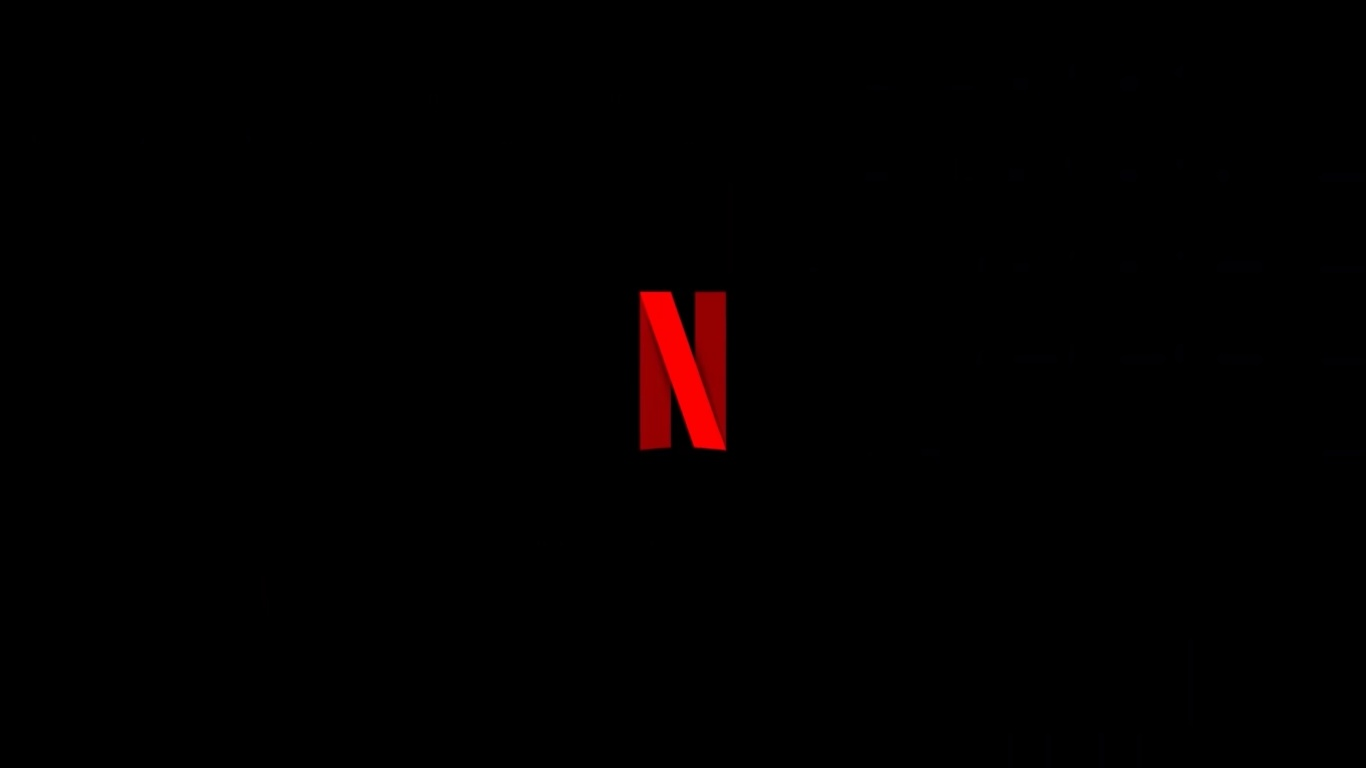
\includegraphics[scale=0.25,keepaspectratio=true]{images/12.jpg}
    \caption{Splash Screen -- Garante fixação da marca}
    \label{pic_12}
\end{figure}

Vantagens para a plataforma ser para os compradores:
\begin{enumerate}
    \item Se torna autoridade como plataforma de consumo e vendas de produtos digitais;
    \item Página de vendas simples e já integrada com a plataforma;
    \item Menor custo e trabalho para o produtor, podendo focar de fato no conteúdo de seus trabalhos;
    \item Divulgação orgânica;
    \item Redução considerável da quantidade de tickets;
    \item Poderíamos fazer parcerias com universidades para melhorar os algoritmos de aprovação de produtos e de sistema de recomendação de dados;
    \item LGPD compliant
    \item PPLD compliant
\end{enumerate}

Ainda existe a possibilidade de atrair o público de entretenimento, o que movimentaria muito GMV. A Figura \ref{pic_13} representa o posicionamento adequado para a empresa:
\begin{figure}[H]
    \centering
    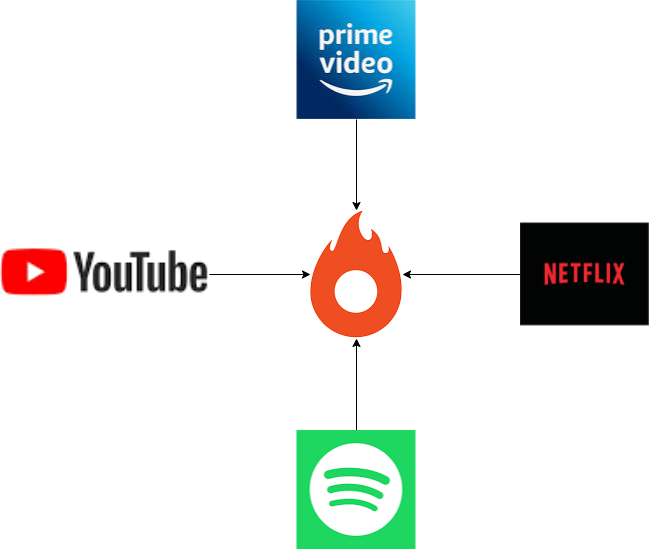
\includegraphics[scale=0.50,keepaspectratio=true]{images/13.png}
    \caption{Posicionamento Global da Hotmart}
    \label{pic_13}
\end{figure}

\begin{itemize}
    \item Usuários insatisfeitos com as políticas de monetização do YouTube podem passar a vender trilhas com baixo custo na nossa plataforma.
    \item Usuários que possuem material como shows ou espetáculos  mas que não conseguem publicar tanto na Amazon Prime quanto na Netflix, poderiam livremente usar nosso espaço para isso.
    \item Cantores e compositores poderiam utilizar de nossa plataforma para vender sua arte e assim por diante,
\end{itemize}

As possibilidades são grandes, time nós temos e força de vontade é o que não me falta para poder contribuir com todas essas mudanças. Caso voê encontre algum erro, tenha alguma dúvida ou queira dar uma sugestão, ficarei muito feliz em receber de braços abertos. No mais, obrigado por ter vindo até aqui.